\documentclass[11pt]{article}

\usepackage[margin=1in]{geometry}
\usepackage{amsmath,amssymb,amsfonts}
\usepackage{booktabs}
\usepackage{xcolor}
\usepackage[colorlinks=true,linkcolor=blue!50!black,urlcolor=blue!50!black]{hyperref}
\usepackage{parskip}
\usepackage{enumitem}
\usepackage{tikz}
\usetikzlibrary{positioning, arrows.meta, calc, fit}

\newcommand{\R}{\mathbb{R}}
\newcommand{\E}{\mathbb{E}}
\newcommand{\KL}{\mathrm{KL}}
\newcommand{\softmax}{\operatorname{softmax}}
\newcommand{\relu}{\operatorname{ReLU}}
\newcommand{\clip}{\operatorname{clip}}
\newcommand{\sg}{\operatorname{stopgrad}}
\newcommand{\Adv}{\hat{A}}
\newcommand{\pol}{\pi_\theta}
\newcommand{\polold}{\pi_{\theta_{\mathrm{old}}}}
\newcommand{\polref}{\pi_{\mathrm{ref}}}

\title{\textbf{Orbit Wars --- RL Formulation and Training Math}}
\author{Native C++/LibTorch stack}
\date{\today}

\begin{document}
\maketitle
\vspace{-1.5em}
\begin{center}\small This document specifies the policy, the reward, and the
training updates used by the native trainer. The trainer supports \emph{two}
algorithms --- \emph{Group Relative Policy Optimization} (GRPO, a group baseline,
Section~\ref{sec:grpo}) and \textbf{PPO\,+\,GAE} (a value-head critic,
Appendix~\ref{sec:ppo}) --- selected by \texttt{TrainConfig::algo}. The current
\texttt{docs/set-ups/1.md} run (the \textbf{v5 target actor} with the redesigned
event reward) trains with \textbf{PPO\,+\,GAE}; GRPO is the alternative.
Symbols map to \texttt{native/rl/config.hpp} and \texttt{native/rl/model/}.\\[0.4em]
\textbf{Leading implementation note.} The actively-developed implementation is the
self-contained pure-PyTorch notebook \texttt{notebooks/setup1\_target\_ppo.ipynb}
(it mirrors the native trunk/reward bit-for-bit). It has since taken the v5 actor
\textbf{three} steps further, all reflected below: (i) the launch fraction $\phi$ is
now a \emph{discrete categorical} (Section~\ref{sec:dist}) --- the whole per-planet
action is discrete, which is the prerequisite for tree search; (ii) destinations the
sun would absorb are \emph{hard-masked} via a reachability mask, and $\phi$ buckets
that cannot launch $\geq 1$ ship are masked too (Section~\ref{sec:dist}); and (iii)
single-snapshot self-play is replaced by an \textbf{Elo/PFSP league}
(Section~\ref{sec:league}), and the hand-coded curriculum stages are \emph{removed} --- the league
\emph{is} the curriculum (Section~\ref{sec:curriculum}). The native C++ stack still carries the continuous-$\phi$
target actor; porting these three is pending. Appendix~\ref{sec:search} maps the
\textbf{AlphaZero/MuZero family} onto this discrete actor --- the planned next step
beyond PPO.\end{center}
\tableofcontents
\bigskip

%==============================================================
\section{Problem setup}\label{sec:problem}
Orbit Wars is an $N$-player symmetric Markov game with $N\in\{2,4\}$. The engine sets
$N=\lvert\text{state}\rvert$ (\texttt{num\_agents}) and assigns $N$ home planets from a
4-fold-symmetric quadrant group ($N=2$: two opposite quadrants; $N=4$: all four). Each turn all
players \emph{simultaneously} issue a set of fleet \emph{launches}; the deterministic engine then
moves fleets, resolves collisions/combat, rotates planets, produces ships, and (on scheduled
steps) spawns comets. Scoring is a \textbf{free-for-all}: at termination player $i$'s score is its
total ship count $\mathrm{ships}_i$ (planets $+$ fleets), and the seat(s) with the maximum score
receive reward $+1$, all others $-1$ (so $N=4$ is winner-take-all among four individuals --- not
teams).

\paragraph{Training scope of this document.} We currently train the \textbf{two-player special
case} ($N=2$: ego $p=0$ against one opponent in the opposite quadrant). The native world generator
places exactly two homes; the shaped reward (Section~\ref{sec:reward}) uses the zero-sum margin
$\mathrm{ships}_0-\mathrm{ships}_1$; and each group plays a single opponent (scripted, or a frozen
snapshot, Section~\ref{sec:league}). The policy (Section~\ref{sec:policy}) and the GRPO update
(Section~\ref{sec:grpo}) are \emph{$N$-agnostic}; lifting to 4-player FFA requires only (i) 4-home
world generation, (ii) replacing the zero-sum margin with the FFA return (max-score seat $+1$ else
$-1$, or a rank-based shaping), and (iii) seating $\geq 1$ extra opponents per game. This 2p$\to$4p
gap is an open modeling item, revisited in Section~\ref{sec:reward}.

\paragraph{Target action space (current --- \texttt{target\_actor}).}
A turn's action is \emph{factored over the $E$ planet slots} of the observation. Per \textbf{owned}
planet $e$ the model emits \textbf{one launch per step}, a pair $(d_e,\varphi_e)$:
\begin{itemize}[nosep]
\item a \textbf{destination} $d_e\in\{1,\dots,E\}$ --- a \emph{categorical} over the $E$ observation
planet slots, masked to the \emph{alive} \textbf{and sun-reachable} planets (the reachability mask of
Section~\ref{sec:dist}), i.e.\ the model picks \emph{which} planet to send to;
\item a \textbf{launch fraction} $\phi_e$ --- the percent of that planet's ships to send. \emph{In the
leading (notebook) actor this is now a \textbf{discrete categorical}} over $N_\phi$ buckets
$\Phi=\{0\%,5\%,10\%,\dots,100\%\}$ (\texttt{PHI\_BINS}, step $5\%$, $N_\phi=21$; bucket $0$ is a no-op),
making the entire per-planet action discrete. (The native stack still emits the older \emph{continuous}
$\phi_e\in(0,1)$ squashed scalar; Section~\ref{sec:dist} gives both.)
\end{itemize}
A \textbf{heuristic} turns the destination into the heading: $\theta_e=\operatorname{atan2}\big(p_y[d_e]-p_y[e],\;p_x[d_e]-p_x[e]\big)$,
a straight line at the destination planet (the ``shortest path''). The model therefore \textbf{never
learns aiming} --- this removes the continuous-aiming learning problem that motivated the earlier
$(d^x,d^y)$ direction-vector design (and its passive-basin failure). A planet \emph{commits} the launch
iff $\phi_e\ge\tau_{\mathrm{act}}$ (\texttt{act\_threshold}$=0.05$; in the discrete actor equivalently
bucket index $\geq 1$), sending $n_e=\lfloor\phi_e\,S_e\rfloor$ ships. The stored action is the pair
$(d_e,\varphi_e)$ --- destination slot and ($\phi$ bucket index, discrete actor / $\phi$ value,
continuous actor) --- so $\texttt{n\_action\_params}=2$ per planet. Because $\phi$ buckets that would
floor to $n_e=0$ ships are masked out (Section~\ref{sec:dist}), the discrete actor essentially never
emits a committed-but-empty launch (the invalid-launch rate fell from ${\sim}20$/step to ${\sim}0$).

The destination categorical is sized to $E=\texttt{planet\_cap}$ (the observation slot count), so the
target actor \textbf{forces} $\texttt{max\_entities}=\texttt{planet\_cap}$: in the GPU env this is
$E=48$ (the build sets \texttt{max\_entities}$\leftarrow$\texttt{planet\_cap} whenever
\texttt{target\_actor} is on). Because the destination is a real planet slot and there is one launch
per planet, the action is \textbf{structurally legal} --- illegal/over-dispatch is essentially gone (no
more spraying), so the old invalid-dispatch-penalty machinery and the ``learn legality from a
penalty / optional action mask'' discussion become moot for this actor.

\paragraph{Superseded continuous actor (\texttt{target\_actor=false}).} The target actor
\emph{supersedes} the earlier \textbf{continuous} actor, which is retained behind the
\texttt{--target-actor} flag (\texttt{target\_actor=false}, the config default). There each slot $e$
emitted a fixed block of $3K$ \emph{continuous} controls ($K=5$ fleet slots, three scalars each), so
the action was a $40\times 15$ matrix $a\in[0,1]^{E\times 3K}$ ($E=40$). Fleet slot $k$ of planet $e$
was a triple $(d^x_{e,k},d^y_{e,k},\phi_{e,k})\in[0,1]^3$: a \emph{direction vector} $(d^x,d^y)$,
recentred to $[-1,1]$ as $2d-1$ and mapped to a launch angle
$\theta_{e,k}=\operatorname{atan2}(2d^y_{e,k}-1,\,2d^x_{e,k}-1)$ ($0$--$360^\circ$, continuous --- no
bins), and a \emph{ship fraction} $\phi_{e,k}$ mapped to $0$--$100\%$ of the launching planet's current
ships. A planet could thus dispatch up to $K=5$ fleets in one step, each to an independently chosen
heading and size; the engine processed the $K$ launches in slot order, deducting ships
\emph{sequentially}. That actor was \textbf{not} masked: it emitted the full $40\times 15$ block every
step and was meant to learn the dynamic legal subset from an invalid-dispatch penalty (the desired
output for a non-existent slot being the zero action; dispatching from an unowned/empty planet or
\emph{over-dispatching} a planet's $K$ fractions past $100\%$ being penalized ``everywhere''). An
optional hard mask (\texttt{action\_mask\_policy}) could instead force the per-planet legal mask
$m_e u_e\mathbf{1}[S_e>0]$ onto the action and drop masked slots from the log-prob/entropy sums; both
the penalty-learned legality and that mask applied \emph{only} to this continuous actor. The continuous
actor's direction-vector parameterization made the heading \emph{linear in relative position} ---
attention over the planet tokens (Section~\ref{sec:policy}) could produce a target-minus-self vector
directly, whereas a linear head cannot turn a relative position into $\operatorname{atan2}(\cdot)$ a
scalar heading would require --- but learning that aiming proved hard, which is precisely what the
target actor sidesteps by emitting a destination slot and aiming via the heuristic above.

%==============================================================
\section{Observation encoding}\label{sec:obs}
For ego player $p$ and state $s$, the encoder (\texttt{native/core/encode.hpp}) emits four arrays:
the per-planet entity matrix $X\in\R^{E\times F}$ ($E=40$ planet slots, $F=32$ features each); the
board-summary globals $g\in\R^{G}$ ($G=10$, a \emph{separate} input --- \textbf{not} replicated into
each row); the entity mask $m\in\{0,1\}^{E}$ ($m_e=1$ iff slot $e$ holds a real entity); and the
action mask $u\in\{0,1\}^{E}$ ($u_e=1$ iff $e$ is an ego-owned planet with $>0$ ships). \emph{Neither
$m$ nor $u$ gates the actor} (Section~\ref{sec:policy}): $m$ only hides padding slots inside the
attention block, and $u$ is \emph{both} an input feature (body row $10$, below) and the key used to
\emph{decode} launches and score the invalid-dispatch penalty (Section~\ref{sec:reward}); the dynamic
legal action subset is otherwise \emph{learned} from that penalty, not hard-masked. Each planet row
$X_e\in\R^{32}$ is $11$ \emph{body} features followed by a $21$-feature \emph{incoming-threat block};
all $32$ are listed exhaustively below.

\paragraph{Per-planet body features (rows $0$--$10$).} Each value is normalized into roughly
$[-1,1]$. Here $S$ is the planet's ship count, $\varrho$ its radius, $d_c$ its distance to board
centre, $\omega$ the board angular velocity, and $\ell(n)=\ln(1+n)/\ln 1000$ the shared ship-count
log-compressor.
\begin{center}\small
\begin{tabular}{@{}clll@{}}
\toprule
\# & Feature & Encoded value & Meaning \\
\midrule
0  & position $x$        & $p_x/100$                            & horizontal position on the $100{\times}100$ board, $[0,1]$ \\
1  & position $y$        & $p_y/100$                            & vertical position, $[0,1]$ \\
2  & orbital speed       & $|\omega|\,d_c/6$ ($0$ if static)    & tangential orbit speed, relative to $v_{\max}{=}6$ \\
3  & spin sign           & $+1$ ccw / $-1$ cw / $0$             & rotation direction; $0$ if stationary or a comet \\
4  & radius              & $\varrho/3$                          & capture / collision disk size \\
5  & production          & $\mathrm{prod}/5$                    & ships made per tick (the reward-defining quantity) \\
6  & ships               & $\ell(S)$                            & garrison size, log-compressed \\
7  & ownership code      & $0$ neu / $1$ ego / $2$--$N$ enemy   & owner, ego-relative (stable under seat rotation) \\
8  & dist.\ to centre    & $d_c/70.71$                          & radial distance from the sun ($70.71{=}\tfrac{\sqrt2}{2}{\cdot}100$, half-diagonal) \\
9  & comet flag          & $\mathbb{1}[\text{comet}]$           & $1$ for a comet, else $0$ \\
10 & action mask $u_e$   & $\mathbb{1}[\text{ego}\wedge S{>}0]$ & $1$ iff ego-owned with ships (also the decode/penalty key) \\
\bottomrule
\end{tabular}
\end{center}

\noindent\emph{Why feed both radius and production?} For a normal planet they are redundant
($\varrho=1+\ln(\mathrm{prod})$), but we feed both so the net need neither invert the $\ln$ nor
re-derive the reward-defining quantity. \emph{Why an explicit comet flag?} A \emph{stationary} body
has speed $0$ and spin sign $0$, but an \emph{orbiting} planet and a \emph{comet} both move, so
velocity alone cannot separate them; the flag also marks where the radius law breaks (a comet carries
the fixed \texttt{COMET\_PRODUCTION}$=1$ at an unrelated radius). The comet's remaining lifetime is
\textbf{deliberately hidden by the engine} (agents may not reconstruct the spawn/expiry schedule), so
this binary flag is the only observable comet signal.

\paragraph{Board-summary globals $g\in\R^{10}$.} One small vector summarising the whole board,
embedded once and broadcast to the action heads (Section~\ref{sec:policy}) rather than copied into
every planet row. With $\Sigma$ a board-wide sum, $n_p$ the planet count, and $\ell$ the same
log-compressor:
\begin{center}\small
\begin{tabular}{@{}cll@{}}
\toprule
\# & Encoded value & Meaning \\
\midrule
0 & $\mathrm{step}/T$                   & game phase (fraction of the $T$-step episode elapsed) \\
1 & $10\,\omega$                        & board angular velocity (orbit rate, scaled) \\
2 & $\ell(\Sigma\,\text{ego ships})$    & ego total garrison ships (log) \\
3 & $\ell(\Sigma\,\text{enemy ships})$  & enemy total garrison ships (log) \\
4 & $n^{\mathrm{ego}}_p/n_p$            & ego share of all planets \\
5 & $n^{\mathrm{enemy}}_p/n_p$          & enemy share of all planets \\
6 & $n^{\mathrm{neutral}}_p/n_p$        & neutral share of all planets \\
7 & $\ell(\Sigma\,\text{ego fleet})$    & ego in-flight (fleet) ships (log) \\
8 & $\ell(\Sigma\,\text{enemy fleet})$  & enemy in-flight (fleet) ships (log) \\
9 & $\min(n_p,E)/E$                     & planet-slot occupancy (how full the $E$ rows are) \\
\bottomrule
\end{tabular}
\end{center}
This game is a \textbf{free-for-all}: there are no allies; an inbound fleet is either the ego's own
(a reinforcement) or an enemy's, distinguished by the owner sign in the threat block (next).

\paragraph{Incoming-fleet threat block (per planet, baked into the row).}\label{sec:threat}
A purely \emph{reactive} policy cannot defend if it cannot see what is coming. For each planet we
therefore bake a compact list of \emph{its own} inbound fleets directly into that planet's feature
row. First we project every in-flight fleet to the planet it will hit, and when. A fleet at
position $o$ with unit heading $\hat d=(\cos\alpha,\sin\alpha)$ and ship count $\nu$ moves at speed
\begin{equation}
v(\nu)=\min\!\Big(v_{\max},\; 1+(v_{\max}-1)\big(\tfrac{\ln \max(1,\nu)}{\ln 1000}\big)^{1.5}\Big),
\qquad v_{\max}=6,
\end{equation}
matching the engine's fleet dynamics. For a planet at $c$ with radius $\varrho$, the ray
$o+t\hat d$ enters the planet disk at
\begin{equation}
t_{\mathrm{ca}} = -\langle o-c,\hat d\rangle,\quad
p^2 = \lVert o-c\rVert^2 - t_{\mathrm{ca}}^2,\quad
t_{\mathrm{hit}} = t_{\mathrm{ca}} - \sqrt{\varrho^2-p^2}\ \ (\text{if } t_{\mathrm{ca}}\!\geq\!0,\ p^2\!\leq\!\varrho^2).
\end{equation}
The fleet is assigned to the planet with the smallest $t_{\mathrm{hit}}\!\geq\!0$ (dropped if the
ray first crosses the central sun --- a \emph{fixed} disk of radius $\mathrm{SUN\_RADIUS}=10$,
constant all game --- or hits nothing), with ETA $\tau=t_{\mathrm{hit}}/v(\nu)$ in ticks.

\subparagraph{Two ranked views per planet (tuneable counts).} Among the fleets assigned to a
planet we keep two short lists: the \texttt{N\_SOON}$=2$ with the smallest ETA (most
\emph{imminent}) and the \texttt{N\_BIG}$=5$ with the largest ship count (most \emph{dangerous});
the lists may overlap. Each of the $7$ slots contributes $3$ features
\begin{equation}
\big[\ \mathrm{sgn},\ \ \tau,\ \ \widetilde\nu\ \big],
\qquad \widetilde\nu=\frac{\ln(1+\nu)}{\ln 1000},
\end{equation}
i.e.\ \emph{who it belongs to} ($\mathrm{sgn}=+1$ ego reinforcement $/-1$ enemy), \emph{arrival
time} as the ETA $\tau$ in ticks (scaled by $1/\texttt{THREAT\_ETA\_SCALE}$, $\texttt{THREAT\_ETA\_SCALE}=100$),
and \emph{ship count} $\widetilde\nu$. Empty slots are all zero --- $\mathrm{sgn}=0$ there already
marks ``no fleet,'' so $\tau=0$ is unambiguous --- giving the row's $7\times 3=21$ threat features,
which occupy entity-row indices $11$--$31$ exactly as:
\begin{center}\small
\begin{tabular}{@{}cl ccc@{}}
\toprule
Slot & Ranked by & $\mathrm{sgn}$ idx & ETA idx & ships idx \\
\midrule
1 & soonest ETA (1st)   & 11 & 12 & 13 \\
2 & soonest ETA (2nd)   & 14 & 15 & 16 \\
3 & largest fleet (1st) & 17 & 18 & 19 \\
4 & largest fleet (2nd) & 20 & 21 & 22 \\
5 & largest fleet (3rd) & 23 & 24 & 25 \\
6 & largest fleet (4th) & 26 & 27 & 28 \\
7 & largest fleet (5th) & 29 & 30 & 31 \\
\bottomrule
\end{tabular}
\end{center}
(slots $1$--$2$ are the \texttt{N\_SOON} soonest-arriving, slots $3$--$7$ the \texttt{N\_BIG}
largest; per slot the three values are $\mathrm{sgn}\in\{+1\ \text{mine},-1\ \text{enemy},0\
\text{empty}\}$, ETA $=\tau/100$ ticks, ships $=\widetilde\nu=\ell(\nu)$).
Because the list is attached to the destination planet's \emph{own} row, that planet
directly sees ``what is coming at \emph{me} --- how soon, how big, and from whom'' --- local
defensive awareness baked into the \emph{observation}, with no separate fleet tokens. (The
\emph{encoder} has no attention; the \emph{policy network} does add one cross-planet attention block,
Section~\ref{sec:policy}, so a planet can read the others' positions to aim \emph{at} them.) The
projection ignores planet rotation but is computed \emph{identically} in C++ and Python (parity-tested
bit-for-bit), so the natively trained policy behaves identically when served from pure Python.

%==============================================================
\section{Policy network $\pi_\theta$}\label{sec:policy}
The network (\texttt{native/rl/model/policy\_net.hpp}) maps the per-planet entity matrix
$X\in\R^{E\times F}$ (body $+$ incoming-threat features, Section~\ref{sec:obs}) to a per-planet
block of action parameters ($\texttt{n\_action\_params}=2$ for the target actor $(d_e,\varphi_e)$;
$3K$ for the superseded continuous actor). The $G=10$ board-summary globals enter through a
\emph{small separate path}: a one-layer embedding $g'=\relu(W_g\,g+b_g)\in\R^{d_g}$ ($d_g=32$),
broadcast to every planet and concatenated at the action heads --- so the trunk itself stays purely
per-planet (per-row). The actor heads carry \textbf{no separate pointer head}; a value head (the PPO
critic) is built \emph{only} when \texttt{use\_value\_head} is set (the \texttt{set-ups/1.md} run is
PPO, so it is built; GRPO needs no critic). Let $d=\texttt{hidden}$.

\paragraph{Trunk pipeline.} The trunk maps the projected rows through, in order: input projection
$\to$ \textbf{one masked cross-planet self-attention block} $\to$ an optional residual GLU block
(variant A) $\to$ $n_{\mathrm{res}}$ pre-LayerNorm residual MLP blocks $\to$ a final LayerNorm. The
projection $h^{(0)}_e=W_{\mathrm{proj}}x_e+b_{\mathrm{proj}}$ and the MLP/GLU blocks are per-row
(weights shared across planets); the attention block is the \emph{only} cross-row mixing.

\smallskip\noindent\textbf{(1) Masked self-attention (the aiming mechanism).} A single-head attention
over the $E$ planet tokens, computed on the pre-LayerNormed tokens $\tilde h=\mathrm{LN}(h^{(0)})$:
\begin{equation}
A = \softmax\!\Big(\tfrac{(\tilde h W_Q)(\tilde h W_K)^{\!\top}}{\sqrt d}
      + \mathcal{M}_{\mathrm{ent}}\Big)\,(\tilde h W_V),\qquad
h^{(1)} = h^{(0)} + A\,W_O,
\end{equation}
where the key-mask $\mathcal{M}_{\mathrm{ent}}[\,\cdot,j]=-\infty$ for \emph{padding} planets
($m_j=0$, the \texttt{entity\_mask}) so live planets never attend to empty slots. This block is what
lets a planet read another planet's \emph{position} and point a launch \emph{at} it --- a purely
per-row trunk cannot represent a targeted heading (it was added precisely to unblock aiming). It is now
\textbf{toggleable} (\texttt{USE\_ATTENTION}, an A/B like \texttt{use\_glu}): when off, the whole block
(its \texttt{attn\_\{q,k,v,o\}} and \texttt{ln\_attn}) is not built and the trunk is \emph{purely
per-planet}. In the \emph{target} actor aiming is already heuristic, so the block's remaining job is
\emph{cross-planet board reasoning} --- comparing candidate destinations' ownership/garrisons/threats to
choose the destination slot --- which makes the ablation meaningful (at $d{=}512$ it is ${\sim}1.05$M of
the ${\sim}5.3$M parameters; the value head still pools over planets either way).

\smallskip\noindent\textbf{(2) Optional residual GLU} (variant A only, \texttt{use\_glu};
Eq.~\ref{eq:glu}, Fig.~\ref{fig:glu}): $h \mathrel{+}= W_o\big((W_v h)\odot\sigma(W_g h)\big)$.

\smallskip\noindent\textbf{(3) Pre-LayerNorm residual MLP blocks} ($n_{\mathrm{res}}$ of them):
$\mathcal M(z)=z+W_b\,\relu\!\big(W_a\,\mathrm{LN}(z)\big)+b_b$, then a \textbf{final LayerNorm}. The
pre-norm is not cosmetic: without it the deep trunk drove the head pre-activations large, the sigmoid
squash saturated, and the aiming gradient vanished --- pre-LN keeps activations bounded so the heads
stay in the squash's responsive range. So
\begin{equation}
h_e = \mathrm{LN}\Big(\big(\underbrace{\mathcal M\circ\dots\circ\mathcal M}_{n_{\mathrm{res}}}\big)
      \big[\,\circ\,\mathcal B_{\mathrm{GLU}}\,\big]\big(h^{(1)}_e\big)\Big)\in\R^{d},
\qquad e=1,\dots,E,
\end{equation}
($\mathcal B_{\mathrm{GLU}}$ present only in variant A; $h^{(1)}$ is the post-attention token). The
\texttt{use\_glu} A/B (GLU vs.\ an extra residual MLP) is the trunk comparison; everything else is identical.
Two masks appear and must not be confused: \texttt{entity\_mask} ($m_e$, live-vs-padding) gates
\emph{attention} above; \texttt{action\_mask} ($u_e\mathbf 1[S_e>0]$, owned-with-ships) gates the
\emph{action} (the optional policy mask, Section~\ref{sec:dist}). The board-wide signal is the small
broadcast embedding $g'$ concatenated at the heads.

\begin{figure}[h]
\centering
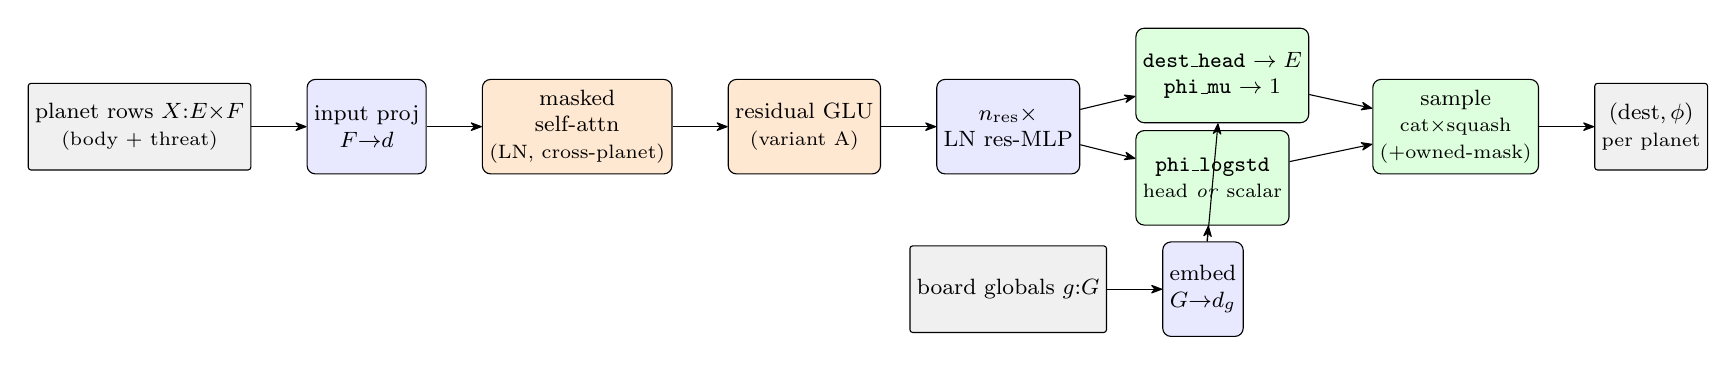
\begin{tikzpicture}[
  font=\footnotesize, >={Stealth[round]}, node distance=5mm and 7mm,
  io/.style ={draw, rounded corners=1pt, fill=gray!12,  align=center, minimum height=11mm, inner sep=2.5pt},
  enc/.style={draw, rounded corners=3pt, fill=blue!9,   align=center, minimum height=12mm, inner sep=2.5pt},
  glu/.style={draw, rounded corners=3pt, fill=orange!18, align=center, minimum height=12mm, inner sep=2.5pt},
  act/.style={draw, rounded corners=3pt, fill=green!13,  align=center, minimum height=12mm, inner sep=2.5pt}]
\node[io]  (x)              {planet rows $X{:}E{\times}F$\\\scriptsize(body $+$ threat)};
\node[enc, right=of x]    (proj) {input proj\\$F{\to}d$};
\node[glu, right=of proj] (attn) {masked\\self-attn\\\scriptsize(LN, cross-planet)};
\node[glu, right=of attn] (glu)  {residual GLU\\\scriptsize(variant A)};
\node[enc, right=of glu]  (res)  {$n_{\mathrm{res}}\times$\\LN res-MLP};
\node[act, right=of res, yshift=6.5mm]  (mu)  {\texttt{dest\_head} $\to E$\\\texttt{phi\_mu} $\to 1$};
\node[act, right=of res, yshift=-6.5mm] (ls)  {\texttt{phi\_logstd}\\\scriptsize head \emph{or} scalar};
\node[act, right=8mm of mu, yshift=-6.5mm] (samp) {sample\\\scriptsize cat$\times$squash\\\scriptsize($+$owned-mask)};
\node[io,  right=of samp] (a)  {$(\text{dest},\phi)$\\\scriptsize per planet};
\node[io, below=9mm of res] (g) {board globals $g{:}G$};
\node[enc, right=of g] (gemb) {embed\\$G{\to}d_g$};
\draw[->] (x)--(proj); \draw[->] (proj)--(attn); \draw[->] (attn)--(glu); \draw[->] (glu)--(res);
\draw[->] (res)--(mu); \draw[->] (res)--(ls);
\draw[->] (g)--(gemb); \draw[->] (gemb)--(mu); \draw[->] (gemb)--(ls);
\draw[->] (mu)--(samp); \draw[->] (ls)--(samp); \draw[->] (samp)--(a);
\end{tikzpicture}
\caption{Policy network data flow. The \textbf{trunk is shared by both actors}; only the heads differ.
Planet rows are projected, then mixed by one \textbf{masked cross-planet self-attention} block
(pre-LayerNorm; \texttt{entity\_mask} hides padding planets) --- the only cross-row step. The result
passes through the shared per-row trunk: variant A inserts one residual GLU block (Fig.~\ref{fig:glu})
before the $n_{\mathrm{res}}$ \emph{pre-LayerNorm} residual MLP blocks (variant B: MLP blocks only),
then a final LayerNorm. The $G$ board globals are embedded separately ($g'$, dim $d_g$) and broadcast
to the heads. \textbf{Target actor (current):} \texttt{dest\_head} maps $[h_e;g']$ to the $E$
destination logits $\ell_e$ and \texttt{phi\_mu}/\texttt{phi\_logstd} to the $\phi$ mean/log-std,
sampled as a destination categorical (masked to alive slots) $\times$ a squashed Gaussian
(Section~\ref{sec:dist}), masked to owned planets, whose sample is the pair $(\text{destination},\phi)$
for planet $e$; a heuristic $\theta=\operatorname{atan2}$ then aims the launch at the chosen destination.
\textbf{Continuous actor (superseded):} a two-layer MLP mean head maps $[h_e;g']$ to the $3K$ means
$\mu_e$ and a switchable second head/vector to the $3K$ log-stds, defining a squashed Gaussian whose
samples are the $K$ fleet triples $(d^x,d^y,\phi)$. A value head (the PPO critic) is built only when
\texttt{use\_value\_head} is set; no pooling, no pointer head.}
\label{fig:arch}
\end{figure}

\paragraph{Residual GLU block.} For an input $z\in\R^{d}$, with three $d\times d$ weight
matrices (gate $W_g$, value $W_v$, output $W_o$),
\begin{equation}
\mathrm{GLU}(z) = \big(W_v z + b_v\big)\odot \sigma\!\big(W_g z + b_g\big),
\qquad
\mathcal{B}(z) = z + W_o\,\mathrm{GLU}(z) + b_o \ \in\R^{d},
\label{eq:glu}
\end{equation}

\begin{figure}[h]
\centering
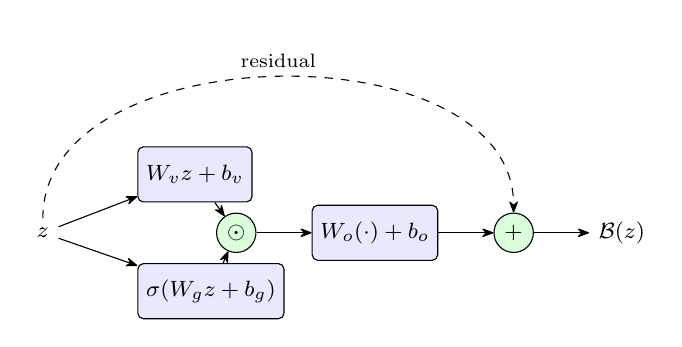
\begin{tikzpicture}[
  font=\footnotesize, >={Stealth[round]},
  lin/.style={draw, rounded corners=2pt, fill=blue!9, minimum height=7mm, inner sep=3pt},
  op/.style ={draw, circle, fill=green!14, inner sep=0.5pt, minimum size=5mm}]
\node (in) {$z$};
\node[lin, above right=2mm and 10mm of in] (val)  {$W_v z + b_v$};
\node[lin, below right=2mm and 10mm of in] (gate) {$\sigma(W_g z + b_g)$};
\node[op,  right=20mm of in] (mul) {$\odot$};
\node[lin, right=7mm of mul] (outp) {$W_o(\cdot) + b_o$};
\node[op,  right=7mm of outp] (add) {$+$};
\node[right=7mm of add] (y) {$\mathcal{B}(z)$};
\draw[->] (in) -- (val); \draw[->] (in) -- (gate);
\draw[->] (val) -- (mul); \draw[->] (gate) -- (mul);
\draw[->] (mul) -- (outp); \draw[->] (outp) -- (add); \draw[->] (add) -- (y);
\draw[->, dashed] (in) to[out=90, in=90] node[above, font=\scriptsize] {residual} (add);
\end{tikzpicture}
\caption{The residual GLU block $\mathcal{B}$ (Eq.~\ref{eq:glu}): a value branch $W_v z$ and a
sigmoid gate $\sigma(W_g z)$ are multiplied elementwise ($\odot$), projected by $W_o$, and added
back to the input (the residual skip). In trunk variant A one such block (its own $d\times d$
weights) follows the input projection, before the residual MLP stack.}
\label{fig:glu}
\end{figure}

where $\sigma$ is the logistic sigmoid and $\odot$ is elementwise. The sigmoid gate lets the
block pass, attenuate, or suppress each feature channel conditionally (e.g.\ amplify the
incoming-threat channels of Section~\ref{sec:threat} when a planet is under attack); the
residual keeps optimization easy. It is applied per planet row and shares weights across rows
just like the rest of the trunk. Whether this gating earns its keep over plain stacked MLPs
(variant A vs.\ B) is exactly the comparison this experiment is set up to answer.

\paragraph{Target-actor heads.} The trunk above is \textbf{unchanged}; only the heads differ. They read
$h'_e=[\,h_e;\,g'\,]\in\R^{d+d_g}$ (trunk token concatenated with the broadcast globals embedding) and
emit, per planet:
\begin{description}[nosep,leftmargin=1.4em]
\item[\texttt{dest\_head}:] a single \texttt{Linear}$(d+d_g\to E)$ producing the destination logits
$\ell_e\in\R^{E}$ (one logit per candidate destination slot). Common to both target actors.
\item[\texttt{phi\_cat} (\emph{discrete actor, leading}):] a single \texttt{Linear}$(d+d_g\to N_\phi)$
producing the $\phi$-bucket logits $h_e\in\R^{N_\phi}$. \emph{Calm init:} weights scaled by
\texttt{init\_mu\_scale}$=0.02$ and the non-no-op bucket biases set to \texttt{init\_phi\_bias}$=-4$ (the
no-op bucket bias $0$), so the policy starts strongly biased to ``no launch'' and a near-uniform
destination, then learns to commit.
\item[\texttt{phi\_mu}/\texttt{phi\_logstd} (\emph{continuous-$\phi$ actor, native}):] \texttt{phi\_mu}
a \texttt{Linear}$(d+d_g\to 1)$ giving the pre-squash mean $\mu_e$ (same calm init), and \texttt{phi\_logstd}
either a \texttt{Linear}$(d+d_g\to 1)$ (state-dependent) or a shared scalar \texttt{phi\_logstd\_param}
(\texttt{std\_state\_dependent}), clipped to $[\varsigma_{\min},\varsigma_{\max}]$.
\end{description}
Exactly one $\phi$ head is built (\texttt{DISCRETE\_PHI}); the continuous $E{\times}3K$ heads below are
\emph{not} built in either target mode. Sampling (destination categorical $\times$ a $\phi$ categorical
or squashed Gaussian) is in Section~\ref{sec:dist}; the decode into engine launches in
Section~\ref{sec:decode}.

\paragraph{Continuous action heads (mean, and a switchable log-std) --- continuous-actor variant.} The heads read
$h'_e=[\,h_e;\,g'\,]\in\R^{d+d_g}$ (trunk token concatenated with the broadcast globals embedding). The
\emph{mean} head is a \textbf{two-layer MLP}, $\mu_e=W_{\mu 2}\,\relu(W_{\mu 1}h'_e+b_{\mu 1})+b_{\mu 2}\in\R^{3K}$
(\texttt{mu\_h1}$\to$ReLU$\to$\texttt{mu\_h2}) --- nonlinear, not a single affine map. The log-std
$\varsigma_e$ is supplied in one
of \textbf{two switchable ways} (\texttt{ModelConfig::std\_state\_dependent}), kept as an explicit
A/B because they trade off expressiveness against training stability:
\begin{description}[nosep,leftmargin=1.4em]
\item[State-dependent (a head):] $\varsigma_e = W_\varsigma\,h_e + b_\varsigma\in\R^{3K}$ --- the
spread depends on the board, so the policy explores where the board is open/uncertain and commits
(small $\sigma$) where the move is forced (e.g.\ a clear defensive launch). More expressive, but
can destabilize (it may drive $\sigma\!\to\!0$ in ``confident'' states and stop exploring).
\item[State-independent (a vector):] $\varsigma_e\equiv\varsigma\in\R^{3K}$, one learnable vector
shared across all planets and states --- the standard, stable PPO default.
\end{description}
Either way, $\sigma_e=\exp\!\big(\clip(\varsigma_e,\varsigma_{\min},\varsigma_{\max})\big)$, the
clip keeping $\sigma$ from collapsing to $0$ or exploding. \textbf{Exploration anneal (explore$\to$exploit
hand-off).} The entropy bonus pushes $\varsigma$ \emph{up} to the cap, so with a fixed cap $\sigma$ pins
at its maximum for the whole run: the sampled action $\varphi(\mu+\sigma\,\varepsilon)$ stays
noise-dominated, the per-trajectory advantage is then $\approx$uncorrelated with the mean, and the
policy-gradient terms \emph{cancel} --- a frozen policy that never exploits (observed empirically:
$\operatorname{adv\_std}=1$ yet $\mathrm{kl}\to0$). The fix is a two-phase schedule on the cap. PHASE~1
(the first \texttt{sigma\_decay\_iters} iterations) \emph{forces} the cap down from $\varsigma_{\max}$ to
$\varsigma_{\max}^{\,\mathrm{end}}$ (e.g.\ $\sigma:1.0\!\to\!0.05$), so the action quickly becomes
mean-determined and the gradient attributable. PHASE~2 releases the cap to
$\varsigma_{\max}^{\,\mathrm{post}}$ (\texttt{logstd\_max\_post}) and hands $\sigma$ to the
state-dependent log-std head, free within $[\,e^{\varsigma_{\min}},\,e^{\varsigma_{\max}^{\,\mathrm{post}}}\,]$
(e.g.\ $[0.01,0.2]$): it re-widens where the board is uncertain and tightens where the move is forced.
(With \texttt{sigma\_decay\_iters}$=0$ the cap instead decays linearly over the whole run, or not at all
if $\varsigma_{\max}^{\,\mathrm{end}}{=}\varsigma_{\max}$.) The mean head and trunk are identical
across the two, only the source of $\varsigma$ differs, and $\varsigma$ is trained by the same
surrogate$+$entropy gradients (Section~\ref{sec:dist}). Each head emits $3K=15$ numbers --- the
per-component parameters of the $K$ fleet triples $(d^x,d^y,\phi)$; sampling and the $[0,1]$ squash
are in Section~\ref{sec:dist}, decoding into engine launches in Section~\ref{sec:decode}. The mean
head is a 2-layer MLP (above) rather than a single linear map --- the extra nonlinearity was added
alongside attention while chasing the aiming gradient; the discrete pointer/target actor of the
previous design is retired together with target mode.

\paragraph{Calm initialization (\texttt{init\_mu\_scale}, \texttt{init\_phi\_bias}).} A deep
from-scratch trunk would otherwise drive the freshly initialised mean head to large, arbitrary
pre-squash values, so the policy would either spray launches everywhere or saturate the squash before
learning anything. Two init knobs tame the start: the final mean-head weights are scaled by
\texttt{init\_mu\_scale}$=0.02$ so every output begins $\approx$ its bias regardless of trunk depth,
and the $\phi$ (ship-fraction) component's bias is set to \texttt{init\_phi\_bias}$=-4$ so
$\varphi(-4)\approx0.018$ --- with the initial $\sigma$ only $\sim$$14\%$ of slots commit a launch at
step~$0$. Less calm (smaller $|\text{bias}|$, larger scale) means more early commits and more mistakes
to learn from; too calm and the policy is inert and learns nothing.

\paragraph{Layer inventory (variant A).} Modules are \texttt{nn.Linear} except the \texttt{ln\_*}
which are \texttt{nn.LayerNorm}. Names match \texttt{policy\_net.cpp}.
\begin{center}\small
\begin{tabular}{@{}lll@{}}
\toprule
Module & Layers (name: shape) & Count \\
\midrule
Input projection & \texttt{proj}:$F{\to}d$ & 1 \\
Self-attention & \texttt{attn\_\{q,k,v,o\}}:$d{\to}d$ & 4 \\
LayerNorm (pre-attn, per-res, final) & \texttt{ln\_attn}, \texttt{ln\_res$i$}, \texttt{ln\_out}:$d$ & $n_{\mathrm{res}}{+}2$ \\
Residual GLU (variant A) & \texttt{glu\_\{gate,val,out\}}:$d{\to}d$ & 3 \\
Residual MLP $\times n_{\mathrm{res}}$ & \texttt{res$i$\{a,b\}}:$d{\to}d$ & $2n_{\mathrm{res}}$ \\
Board-globals embed & \texttt{g\_embed}:$G{\to}d_g$ & 1 \\
\midrule
\multicolumn{3}{@{}l@{}}{\emph{Target actor (current):}}\\
Destination head & \texttt{dest\_head}:$d{+}d_g{\to}E$ & 1 \\
$\phi$ bucket head \emph{(discrete, leading)} & \texttt{phi\_cat}:$d{+}d_g{\to}N_\phi$ & 1 \\
$\phi$ mean head \emph{(continuous, native)} & \texttt{phi\_mu}:$d{+}d_g{\to}1$ & 1 \\
$\phi$ log-std (switchable, continuous) & \texttt{phi\_logstd}:$d{+}d_g{\to}1$ \ \emph{or} scalar \texttt{phi\_logstd\_param} & 1 \\
\midrule
\multicolumn{3}{@{}l@{}}{\emph{Continuous actor (superseded):}}\\
Mean head (MLP) & \texttt{mu\_h1}:$d{+}d_g{\to}d$, \texttt{mu\_h2}:$d{\to}3K$ & 2 \\
Log-std (switchable) & \texttt{logstd\_head}:$d{+}d_g{\to}3K$ \ \emph{or} vector $\varsigma{:}3K$ & 1 \\
\midrule
Value head (PPO only): in-proj & \texttt{val\_in}:$d{+}d_g{\to}d$ & $0$/$1$ \\
\quad residual MLP $\times$\,\texttt{VALUE\_RES\_BLOCKS} & \texttt{val\_res\{a,b\}}:$d{\to}d$, \texttt{val\_ln}:$d$ & $3\,n_v$ \\
\quad readout & \texttt{val\_out}:$d{\to}1$ & $0$/$1$ \\
\bottomrule
\end{tabular}
\end{center}
\noindent No pointer head. The value head (the critic) is built \emph{only} when
\texttt{use\_value\_head} is set --- it is present for the PPO\,+\,GAE run (\texttt{set-ups/1.md}) and
absent for GRPO. Exactly one actor's heads are built, selected by \texttt{target\_actor}. Variant B
replaces the GLU block with an extra residual MLP block (no gating). With $F{=}32$ ($11$ body $+$ $21$
threat), $G{=}10$, $d_g{=}32$, and the \texttt{set-ups/1.md} target-actor scale $d{=}512$,
$n_{\mathrm{res}}{=}6$ this is on the order of a few~M parameters. The pure-Python serving twin
(\texttt{orbit\_wars\_rl/agents/ppo\_policy.py}) must mirror this trunk, board path, and heads
bit-for-bit for the Kaggle submission to reproduce the natively trained policy; it serves the actor
only (no critic at inference).

%==============================================================
\section{Action distribution}\label{sec:dist}
For the \textbf{target actor}, the per-planet action is the pair $(d_e,\varphi_e)$, \emph{independent
across planets} given $s$. The \textbf{leading actor} (\texttt{DiscreteTargetDist}) makes \emph{both}
factors categorical --- the destination over planet slots and $\varphi$ over the $N_\phi$ buckets
$\Phi=\{0,0.05,\dots,1\}$ --- so the entire action is discrete. Two structural \textbf{masks} encode
heuristics the model would otherwise have to relearn:
\begin{description}[nosep,leftmargin=1.4em]
\item[Reachability $R_{e,j}$ (sun occlusion).] A straight shot $e\!\to\!j$ is absorbed by the central
sun (disk centre $c_\odot$, fixed radius $r_\odot{=}10$) iff the segment crosses that disk before
reaching $j$. With $\hat u=(p_j-p_e)/\lVert p_j-p_e\rVert$, $t=\langle c_\odot-p_e,\hat u\rangle$,
$p^2=\lVert c_\odot-p_e\rVert^2-t^2$, the shot is blocked iff $t\ge0$, $p^2\le r_\odot^2$, and
$0\le t-\sqrt{r_\odot^2-p^2}<\lVert p_j-p_e\rVert$ (the \emph{same} ray/disk projection as the threat
encoder, Section~\ref{sec:threat}). Then $R_{e,j}=\mathbb 1[\text{not blocked}]$, with $R_{e,e}=1$.
$R$ is recomputed from the encoded positions ($p_x,p_y$ = body rows $0,1$), so it is identical in
rollout and update with \emph{no} extra trajectory buffers.
\item[$\phi$-bucket validity $\mathcal V_{e,b}$.] Bucket $b$ is usable for planet $e$ iff it launches at
least one ship, $\lfloor \Phi_b\,S_e\rfloor\ge 1$; the no-op bucket $b{=}0$ is always kept. $S_e$ is
recovered (and rounded) from the log-ship feature (row $6$), again consistent across rollout/update.
\end{description}
The two masked factors are
\begin{align}
d_e &\sim \mathrm{Cat}\big(\softmax(\tilde\ell_e)\big),
  & \tilde\ell_{e,j} &= \ell_{e,j}\ \text{if } (m_j{\wedge}R_{e,j}),\ \text{else } -\infty,\\
b_e &\sim \mathrm{Cat}\big(\softmax(\tilde h_e)\big),\quad \varphi_e=\Phi_{b_e},
  & \tilde h_{e,b} &= h_{e,b}\ \text{if } \mathcal V_{e,b},\ \text{else } -\infty,
\end{align}
where $\ell_e,h_e$ are the \texttt{dest\_head}/\texttt{phi\_cat} logits. The joint log-probability and
entropy sum over \textbf{owned} planets only (unowned planets are forced to the no-op action $(d{=}0,b{=}0)$
and excluded):
\begin{equation}
\log\pol(a\mid s) = \sum_{e:\,\text{owned}}
\Big[\,\log\softmax(\tilde\ell_e)[d_e] \;+\; \log\softmax(\tilde h_e)[b_e]\,\Big],
\label{eq:logp}
\end{equation}
\begin{equation}
\mathcal{H}\big[\pol(\cdot\mid s)\big] = \sum_{e:\,\text{owned}}
\Big[\,\mathcal H_{\mathrm{cat}}\big(\softmax(\tilde\ell_e)\big) + \mathcal H_{\mathrm{cat}}\big(\softmax(\tilde h_e)\big)\,\Big].
\label{eq:ent}
\end{equation}
At evaluation the policy is greedy, $d_e=\arg\max_j\tilde\ell_{e,j}$ and $b_e=\arg\max_b\tilde h_{e,b}$
(no sampling). Discretizing $\varphi$ is what makes the action set finite and enumerable per factor ---
the prerequisite for the search-based policy improvement of Appendix~\ref{sec:search}.

\paragraph{Continuous-$\phi$ target variant (native, \texttt{TargetActorDist}).} The native stack keeps
$\varphi_e$ a \emph{squashed Gaussian}: $\varphi_e=\varphi(z_e)$, $z_e\sim\mathcal N(\mu_e,\sigma_e^2)$,
$\sigma_e=e^{\varsigma_e}$, $\varphi(z)=1/(1+e^{-z})$. Its $\phi$ contribution to Eq.~\eqref{eq:logp}
is $\log\mathcal N(z_e;\mu_e,\sigma_e^2)-\log(\varphi_e(1-\varphi_e))$ (the last term the squash
Jacobian, $z_e=\operatorname{logit}\varphi_e$), and to Eq.~\eqref{eq:ent} is $\varsigma_e+\tfrac12\log2\pi e$;
the destination factor and the owned-planet masking are identical. Greedy uses $\varphi_e=\varphi(\mu_e)$.
The reachability mask $R$ applies here too (it gates only the destination factor); $\phi$-bucket validity
is discrete-only. The owned-planet mask is \emph{always} applied for either target actor (replacing the
$E{\times}3K$ actor's ``sum over all slots, invalid-penalty drives unowned to no-op'' rule).

\paragraph{Continuous actor (superseded).} The retired continuous actor was a \textbf{squashed diagonal
Gaussian} over the $E\times 3K$ controls. For each component $a_{e,k,j}$ ($j\in\{d^x,d^y,\phi\}$) the
network emitted a mean $\mu_{e,k,j}$ and log-std $\varsigma_{e,k,j}$, drew $z_{e,k,j}\sim\mathcal
N(\mu,\sigma^2)$ with $\sigma=e^{\varsigma}$, and squashed $a_{e,k,j}=\varphi(z_{e,k,j})$. With the
components conditionally independent, $\log\pol(a\mid s)=\sum_{e,k,j}\big[\log\mathcal
N(z_{e,k,j};\mu,\sigma^2)-\log(a_{e,k,j}(1-a_{e,k,j}))\big]$ and $\mathcal
H=\sum_{e,k,j}(\varsigma_{e,k,j}+\tfrac12\log2\pi e)$. There the sums ran over \emph{all} $E$ slots
(no mask), the invalid-dispatch penalty --- not a mask --- driving non-existent/unowned slots toward
``no launch,'' unless the optional \texttt{action\_mask\_policy} forced
$m_e u_e\mathbf 1[S_e>0]$ and dropped masked slots from both sums. The Gaussian was over the Cartesian
direction $(d^x,d^y)$, so there was no $0/360^\circ$ wrap discontinuity.

\paragraph{How the destination and $\phi$ heads are learned (no separate target).} No head has
labels; all are trained \emph{only} by the policy-gradient surrogate (PPO\,+\,GAE for the current run,
Appendix~\ref{sec:ppo}; or GRPO, Section~\ref{sec:grpo}) and the entropy bonus, through the dependence
of $\log\pol$ on them. The \textbf{destination logits} get the standard policy-gradient
$\partial\log\softmax(\tilde\ell_e)[d_e]/\partial\ell_e=\mathrm{onehot}(d_e)-\softmax(\tilde\ell_e)$, so
an advantage step pushes mass toward the destination chosen when $\Adv>0$ and away when $\Adv<0$. The
\textbf{$\phi$ mean/log-std} story is the squashed-Gaussian one below. Per component, with the
standardized sample $u=(z-\mu)/\sigma$,
\begin{equation}
\frac{\partial \log\mathcal N}{\partial \mu}=\frac{u}{\sigma},
\qquad
\frac{\partial \log\mathcal N}{\partial \varsigma}=u^2-1
\quad(\text{since }\sigma=e^{\varsigma}).
\end{equation}
A policy-gradient step moves each parameter along $\Adv\cdot\partial\log\pol/\partial(\cdot)$ (plus
the entropy term), where $\Adv$ is the GAE per-step advantage (PPO) or the group-relative advantage
(GRPO). For the \textbf{$\phi$ mean}: a sampled $\phi$ that beat its baseline ($\Adv>0$)
pulls $\mu$ toward the fraction taken, one that underperformed pushes it away. For the
\textbf{log-std}: the factor $u^2-1$ is positive when the draw landed \emph{far} from the mean
($|z-\mu|>\sigma$) and negative when \emph{close}, so a far-out action that \emph{helped} ($\Adv>0$)
\textbf{widens} $\sigma$ (explore more there), a far-out action that \emph{hurt} \textbf{narrows} it
(exploit), and a near-mean action that helped also narrows it (commit to the good mean). The entropy
bonus adds a constant $+c_{\mathcal H}$ to the log-std gradient ($\partial\mathcal H/\partial\varsigma=1$),
a steady upward pressure against premature collapse of $\sigma$. Because $\varsigma_e=W_\varsigma h_e$
is produced by the log-std head, these gradients flow on into $W_\varsigma$ and the shared trunk ---
that is how the network learns \emph{where} on the board to be exploratory versus decisive. (In the
state-independent variant the same gradients instead accumulate over all slots into the one shared
$\varsigma$, tuning a single global exploration scale.) Adam applies the update; $\varsigma$ is
clipped to $[\varsigma_{\min},\varsigma_{\max}]$ for numerical safety.

\paragraph{Decode: action $\to$ engine launch.}\label{sec:decode}
\textbf{Target actor.} For each ego-owned planet $e$ (ownership $u_e=1$, ships $S_e>0$) the single
sampled pair $(d_e,\varphi_e)$ decodes to one launch: heading
$\theta_e=\operatorname{atan2}\big(p_y[d_e]-p_y[e],\,p_x[d_e]-p_x[e]\big)$ (straight at the chosen
destination) and $n_e=\lfloor\varphi_e\,S_e\rfloor$ ships, committed iff $\varphi_e\ge\tau_{\mathrm{act}}$
and executed when $n_e\ge 1$ and ships remain. In the \emph{discrete} actor the fraction is the bucket
lookup $\varphi_e=\Phi_{b_e}$ and ``committed'' means $b_e\ge 1$; the $\phi$-validity mask
(Section~\ref{sec:dist}) already guarantees $n_e\ge 1$ for any committed bucket. Since each planet
launches at most once at a real, sun-reachable destination, over-dispatch and phantom/unowned launches
do not arise.
\textbf{Continuous actor (superseded).} There the $K$ fleet triples were emitted in slot order; fleet
$k$ launched $n_{e,k}=\lfloor\phi_{e,k}\,S_e\rfloor$ ships at angle
$\theta_{e,k}=\operatorname{atan2}(2d^y_{e,k}-1,\,2d^x_{e,k}-1)$, the engine deducting ships
\emph{sequentially}; committed fleets that failed to execute (phantom slots, unowned planets, or past
the ship budget) were exactly the $x_t$ counted by that actor's invalid-dispatch penalty.

%==============================================================
\section{Reward and return}\label{sec:reward}
The current \texttt{set-ups/1.md} reward is an \textbf{event-based} reward with \emph{four} channels ---
outcome, capture, dispatch, and a production milestone --- that \textbf{entirely replaces} the legacy
production-shaping reward (the production-margin term $P$, the valid-launch carrot $V$, the miss-penalty
stick $M$, the invalid-dispatch penalty $I$, and the enemy-suppression term $S$ are all \emph{off} in
this run: \texttt{prod\_reward\_weight}, \texttt{valid\_launch\_reward}, \texttt{miss\_launch\_penalty},
\texttt{illegal\_launch\_penalty}, \texttt{enemy\_growth\_weight} are all set to $0$). The four live
channels (\texttt{RolloutConfig}, used identically by the CPU and GPU rollouts of
Section~\ref{sec:gpuenv}) are:

\paragraph{1. Outcome $O$ --- a flat-then-decaying ``flip of winning.''} At termination the game is
scored by total ships ($o_i=+1$ win, $0$ draw, $-1$ loss). The outcome is worth $\pm 1000$
(\texttt{win\_bonus}$=$\texttt{loss\_penalty}$=1000$), held \textbf{flat for the first $100$ steps} and
then \emph{decaying symmetrically} thereafter. With episode length $L$ and
$\delta_{\mathrm o}=$\texttt{win\_decay}$=$\texttt{loss\_decay}$=0.995$ and
$L_0=$\texttt{decay\_start\_step}$=100$,
\begin{equation}
O = \operatorname{sign}(\text{margin})\cdot 1000\cdot \delta_{\mathrm o}^{\,\max(0,\,L-L_0)}.
\label{eq:return}
\end{equation}
The symmetric decay is a ``flip of winning'': it rewards a \emph{decisive} game without making a slow
loss cheaper than a fast one in the opening (both win and loss are flat through the first $L_0$ steps,
so an early scramble is never penalized for taking time). Draw is $0$. The outcome applies in
\emph{all} stages of the $4$-stage curriculum (Section~\ref{sec:curriculum}).

\paragraph{2. Capture $C$.} $+30$ for each ego planet \emph{gained} this step and $-30$ for each planet
\emph{lost} (an owner flip to/from ego among alive slots), with $w_{\mathrm c}=$\texttt{capture\_reward}$=30$:
\begin{equation}
C_t = w_{\mathrm c}\,\big(\#\text{gained}_t - \#\text{lost}_t\big).
\end{equation}

\paragraph{3. Dispatch $D$ --- a bounded ``get moving'' carrot.} $+1$ for each of the \textbf{first $50$
\emph{valid} launches} of the game --- a committed launch whose straight-line heading actually lands on
a planet (the same closed-form ray-vs-disk projection, with sun occlusion, used for the threat features
of Section~\ref{sec:threat}). With $w_{\mathrm d}=$\texttt{dispatch\_reward}$=1$ and budget
$N_{\mathrm d}=$\texttt{dispatch\_count}$=50$, and $\sum_{<t}v$ the valid launches so far,
\begin{equation}
D_t = w_{\mathrm d}\cdot\min\!\big(v_t,\ \max(0,\ N_{\mathrm d}-\textstyle\sum_{<t}v)\big).
\end{equation}
(It counts \emph{valid} launches, not all launches: ships thrown into empty space earn nothing.)

\paragraph{4. Production milestone $P$ --- bring back the economy reward.} $+20$ each time the ego's
\textbf{total ship count} (planets $+$ in-flight fleets), $s$, crosses a \emph{doubling} threshold
starting at \texttt{prod\_milestone\_base}$=100$ (i.e.\ $100,200,400,\dots$). Let the milestone level be
\begin{equation}
m(s) = \big\lfloor \log_2(s/\mathrm{base})\big\rfloor + 1 \ \ (s\ge\mathrm{base}),\qquad m(s)=0\ \ (s<\mathrm{base}),
\end{equation}
and let $m_{\mathrm{prev}}$ be the highest level reached so far. The step reward is
$P_t = w_{\mathrm m}\cdot\max(0,\ m(s_t)-m_{\mathrm{prev}})$ with $w_{\mathrm m}=$\texttt{prod\_milestone\_reward}$=20$,
then $m_{\mathrm{prev}}\leftarrow\max(m_{\mathrm{prev}},\,m(s_t))$. The $\max(0,\cdot)$ and the monotone
$m_{\mathrm{prev}}$ make it \textbf{monotonic}: \emph{losing} ships never claws reward back, so the
channel cleanly rewards a growing economy. The old ``fleet hits a planet'' reward is \textbf{dropped}
--- it rewarded ship depletion (anti-win).

\paragraph{Algorithm: PPO\,+\,GAE per-step assembly.} The \texttt{set-ups/1.md} run trains with
\textbf{PPO\,+\,GAE} (a value-head critic and GAE, Appendix~\ref{sec:ppo}), \emph{not} GRPO. The
per-step reward is the sum of the three dense channels, $r_t = C_t + D_t + P_t$, while the outcome $O$
is \emph{scattered onto the episode's last active step} (so GAE propagates it backward as a return,
rather than a flat offset). Both $r_t$ and $O$ are divided by
$\sigma_R=$\texttt{reward\_scale}$=$\texttt{ppo\_reward\_scale}$=100$ before GAE, which shrinks the value
targets to a fittable range for the MSE critic; advantages are re-normalized afterward, so the policy
objective is unchanged. The per-game return is
\begin{equation}
R = O + C + D + P,\qquad C=\textstyle\sum_t C_t,\ \ D=\textstyle\sum_t D_t,\ \ P=\textstyle\sum_t P_t.
\end{equation}
(The GRPO path of Section~\ref{sec:grpo} would instead broadcast the group-normalized $R$ to every step;
the same four channels feed it, but PPO is the algorithm for this run.)

\paragraph{Legacy production-shaping reward (off in this run).} For reference, the previous reward was a
\emph{smooth bounded} per-game form $R_i=O_i+P_i+V_i-I_i-M_i+S_i$ with: a capped production-margin term
$P=\clip(\sum_t\delta_\Pi^{\,t}\gamma^t w_\Pi\Delta\Pi_0(t),\pm P_{\max})$ on ego production
$\Pi_0(s)=\sum_{p:\mathrm{owner}=0}\mathrm{prod}(p)$; a capped valid-launch \emph{carrot}
$V=\clip(\sum_t\gamma^t w_{\mathrm v}v_t,0,V_{\max})$; an uncapped invalid-dispatch penalty
$I=\sum_t\gamma^t\rho\,x_t$ on committed-but-failed launches $x_t$ (the continuous actor's legality
signal); an uncapped \emph{miss} stick $M=\sum_t\gamma^t\rho_{\mathrm m}m_t$ on legal launches that land
on nothing ($m_t=$ executed $-$ valid); and an enemy-suppression term
$S=-\sum_{t\ge x_0}\gamma^t w_{\mathrm e}y_t$ that rewarded bending the opponent's production growth
down. All of these carry weight $0$ in the current run and are listed only for completeness; their
config knobs survive in \texttt{RolloutConfig}.

\paragraph{Note --- 2p vs.\ 4p objective.} The outcome $O$ (and the implicit margin) are the
two-player ($N=2$) zero-sum forms. In $N=4$ free-for-all the objective is \emph{ordinal} --- be the
maximum of four --- which is not zero-sum: $\operatorname{sign}(\text{margin})$ would become the FFA
win/lose of Section~\ref{sec:problem} (max-score seat $+1$ else $-1$, or a rank-based shaping). The
algorithm machinery (advantage, surrogate, KL) is unchanged --- only $R$ in Eq.~\eqref{eq:return} is
redefined.

%==============================================================
\section{Curriculum (leading: none --- the Elo league \emph{is} the curriculum)}\label{sec:curriculum}
\textbf{The leading implementation has no hand-coded stages.} Every iteration the opponent is
PFSP-sampled from the Elo league (Section~\ref{sec:league}) over \emph{all} pool members --- the two
scripted anchors (\texttt{random}, \texttt{starter}) plus the historical snapshots --- so the schedule
\emph{emerges from skill}. The learner starts rated at the \texttt{random} anchor ($\mathrm{ELO\_INIT}=0$)
and PFSP feeds it the nearest-rated opponents, so it practices against \texttt{random} first, shifts to
\texttt{starter} as its rating climbs past it, then to ever-stronger snapshots --- reproducing the old
stage progression organically, with no boundaries to tune. The only schedule knobs left are
\texttt{TOTAL\_ITERS}, the snapshot cadence \texttt{SELFPLAY\_REFRESH}, and a short
\texttt{SNAPSHOT\_WARMUP} that keeps the pool anchors-only until the learner is worth snapshotting. All
opponents share the one reward of Section~\ref{sec:reward} (the outcome $O$ always applies), and the Elo
update happens every iteration regardless of which opponent was drawn.

\paragraph{Legacy native 4-stage schedule.} The native trainer still uses a \textbf{4-stage,
iteration-driven} curriculum (enabled by \texttt{stage3\_iters}$>0$): the stage advances by
\emph{iteration count} and only the \textbf{opponent} changes. With its flags (\texttt{stage1\_iters}$=0$,
\texttt{stage2\_iters}$=100$, \texttt{stage3\_iters}$=300$, \texttt{total\_iters}$=1400$): Stage~1 (noop)
skipped; Stage~2 vs.\ \texttt{random} (iters $1$--$100$); Stage~3 vs.\ \texttt{starter} (iters
$101$--$400$); Stage~4 self-play$+$starter$+$random (iters $401$--$1400$, drawn $50/25/25$ via
\texttt{selfplay\_prob}$=0.5$). Its self-play opponent is a single \emph{frozen snapshot}
(\texttt{clone\_frozen}), rebuilt on Stage-4 entry and refreshed every \texttt{ckpt\_every\_late}$=100$
iters --- a lagging mirror. The notebook's league/no-stages design supersedes this (the explicit stages
become PFSP weight over the same opponents); the legacy step-fraction $3$-stage schedule remains
available when \texttt{stage3\_iters}$=0$.

%==============================================================
\section{GRPO update}\label{sec:grpo}
GRPO is the trainer's \emph{alternative} algorithm (the \texttt{set-ups/1.md} run uses PPO\,+\,GAE,
Appendix~\ref{sec:ppo}). It replaces the value baseline of actor--critic methods with a
\emph{group-relative} baseline: the policy plays a group of trajectories from the \emph{same} start
against the \emph{same} opponent, and each trajectory's return is centered against its group.

\subsection{Grouped sampling}
For iteration we draw $N$ groups (\texttt{num\_groups}); group $j$ fixes an initial state
$s_0^{(j)}$ (a world) and an opponent, and rolls out $G$ trajectories (\texttt{group\_size})
under the current behavior policy $\polold$ (stochastic). The only within-group variation is
the policy's own action sampling, so the group mean is a valid, low-variance baseline. The
env count is $N\cdot G$ (\texttt{num\_envs}). For every transition we store
$(X,m,u,g)$, the action $a_{i,t}$, the behavior log-prob $\log\polold(a_{i,t}\mid s_{i,t})$,
and the reference log-prob $\log\polref(a_{i,t}\mid s_{i,t})$ (Section~\ref{sec:kl}).

\subsection{Group-relative advantage (no critic)}
Let $\mathcal{G}_j$ be the trajectories of group $j$, with mean and standard deviation
\begin{equation}
\mu_j = \frac{1}{G}\sum_{i\in\mathcal{G}_j} R_i,
\qquad
\varsigma_j = \sqrt{\frac{1}{G}\sum_{i\in\mathcal{G}_j}(R_i-\mu_j)^2}.
\end{equation}
The advantage of trajectory $i$ (group $j=j(i)$), \emph{broadcast to all of its timesteps}, is
\begin{equation}
\boxed{\;
\Adv_i =
\begin{cases}
\dfrac{R_i-\mu_j}{\varsigma_j+\varepsilon}, & \text{whiten\_advantage = true},\\[1.2em]
R_i-\mu_j, & \text{otherwise,}
\end{cases}
\;}
\label{eq:adv}
\end{equation}
with floor $\varepsilon=$\texttt{adv\_eps}. There is no learned $V(s)$ and no temporal-difference
or GAE term --- the entire baseline is Eq.~\eqref{eq:adv}.

\subsection{Clipped policy surrogate}
With the per-step importance ratio
\begin{equation}
\rho_{i,t}(\theta) = \exp\!\Big(\log\pol(a_{i,t}\mid s_{i,t}) - \log\polold(a_{i,t}\mid s_{i,t})\Big),
\end{equation}
(each log-prob the entity sum of Eq.~\eqref{eq:logp}), the surrogate is the PPO clip objective
\begin{equation}
\mathcal{L}^{\mathrm{clip}}(\theta) =
-\,\frac{1}{\sum_i T_i}\sum_{i,t}
\min\!\Big(\rho_{i,t}\,\Adv_i,\ \ \clip(\rho_{i,t},\,1-\epsilon,\,1+\epsilon)\,\Adv_i\Big),
\label{eq:clip}
\end{equation}
with clip range $\epsilon=$\texttt{clip}.

\subsection{KL anchor to a reference policy}\label{sec:kl}
A reference policy $\polref$ (the fixed behavior-cloning checkpoint) anchors training, which
counteracts the empirically observed drift of plain PPO away from the strong BC behavior. We
penalize the unbiased, non-negative $k_3$ estimator of $\KL(\pol\,\|\,\polref)$. With
$\Delta_{i,t}=\log\polref(a_{i,t}\mid s_{i,t})-\log\pol(a_{i,t}\mid s_{i,t})$,
\begin{equation}
\widehat{\KL}_{i,t} = \exp(\Delta_{i,t}) - \Delta_{i,t} - 1 \ \ (\geq 0),
\qquad
\mathcal{L}^{\mathrm{KL}}(\theta) = \frac{1}{\sum_i T_i}\sum_{i,t}\widehat{\KL}_{i,t}.
\label{eq:kl}
\end{equation}

\subsection{Total objective}
Combining the surrogate, the KL anchor (weight $\beta=$\texttt{kl\_beta}) and an entropy bonus
(weight $c_{\mathcal H}=$\texttt{ent\_coef}, from Eq.~\eqref{eq:ent}):
\begin{equation}
\boxed{\;
\mathcal{L}(\theta) =
\mathcal{L}^{\mathrm{clip}}(\theta)
\;+\; \beta\,\mathcal{L}^{\mathrm{KL}}(\theta)
\;-\; c_{\mathcal H}\,\overline{\mathcal{H}}\big[\pol\big]
\;}
\label{eq:loss}
\end{equation}
where $\overline{\mathcal H}$ is the mean entropy over transitions.

\subsection{Optimization}
For each iteration: collect the grouped trajectories under $\polold=\pol$; compute returns
\eqref{eq:return} and advantages \eqref{eq:adv}; then for \texttt{update\_epochs} passes over
\texttt{minibatches} shuffled minibatches, take Adam steps on \eqref{eq:loss} with learning
rate $\eta=$\texttt{lr}, $\epsilon_{\mathrm{Adam}}=$\texttt{adam\_eps}, and global gradient-norm
clip \texttt{max\_grad\_norm}. Advantages are computed once per iteration (off $\polold$); the
ratio \eqref{eq:clip} and KL \eqref{eq:kl} are recomputed each minibatch under the live $\pol$.

%==============================================================
\section{Self-play league (Elo / PFSP)}\label{sec:league}
The leading implementation replaces single-snapshot self-play with a \textbf{rated league} (notebook
\texttt{League}). The pool holds two \emph{anchored} scripted opponents (\texttt{random} at fixed Elo
$0$, \texttt{starter} at fixed Elo $600$ --- they pin the rating scale) plus a growing set of
\emph{frozen policy snapshots}, each with a floating rating $r_m$; the learner carries its own rating
$r_\theta$.

\paragraph{Opponent sampling (PFSP --- the whole pool, every iteration).} There are no stages: at
\emph{every} iteration the single rollout opponent is drawn from \emph{all} pool members $m$ (anchors
\emph{and} snapshots) by \emph{prioritized fictitious self-play}, with weight $w_m=f(p_m)+\epsilon_0$,
where
\begin{equation}
p_m=\Big(1+10^{(r_m-r_\theta)/400}\Big)^{-1}
\end{equation}
is the learner's expected score against $m$ (the logistic Elo expectation) and $f$ is the PFSP curve ---
$f(p)=p(1-p)$ (\texttt{PFSP\_MODE="even"}, default: prefer near-equal opponents) or $f(p)=(1-p)^{P}$
(\texttt{"hard"}: prefer opponents not yet beaten) --- with a uniform floor $\epsilon_0$
(\texttt{PFSP\_FLOOR}) on every member for anti-forgetting (so the scripted anchors keep a residual
probability even once the learner has outgrown them). This single weighting is what makes the Elo ladder
double as the curriculum (Section~\ref{sec:curriculum}): a low-rated fresh learner gets the nearest
anchors, a high-rated one gets the strong snapshots. \textbf{One} opponent is used per rollout, so the
ego win$+\tfrac12$draw fraction over the batch is a clean match score $S\in[0,1]$. (The earlier
\texttt{selfplay\_prob} snapshot-vs-anchor split is retired --- the unified PFSP weight subsumes it.)

\paragraph{Elo update.} After \emph{every} rollout against the drawn opponent $m$, with K-factor $K$
(\texttt{ELO\_K}$=32$ --- raised from $16$ now that Elo \emph{drives} sampling and so must track skill
quickly),
\begin{equation}
r_\theta \leftarrow r_\theta + K\,(S-p_m),\qquad
r_m \leftarrow r_m - K\,(S-p_m)\ \ (\text{anchored }r_m\text{ frozen}).
\end{equation}
Because the learner starts at the \texttt{random} anchor's rating and is updated against whatever it
plays from iteration~0, $r_\theta$ self-calibrates and climbs the ladder. The update is zero-sum and the
fixed anchors pin the absolute scale, so $r_\theta$ is an interpretable, drift-free skill curve (logged
$+$ plotted alongside win rate).

\paragraph{Pool management.} After a short anchors-only warmup (\texttt{SNAPSHOT\_WARMUP} iters, so the
pool is not seeded with a useless random-init net) the learner is snapshotted into the pool every
\texttt{SELFPLAY\_REFRESH} iters (the new snapshot inherits $r_\theta$); auto-snapshots are FIFO-pruned
to \texttt{LEAGUE\_MAX\_SNAPSHOTS}. Externally supplied checkpoints (\texttt{LEAGUE\_INIT\_CKPTS}) are
\emph{pinned} (never pruned), letting past weights seed the pool. Snapshots live on CPU; only the sampled
opponent is moved to the GPU for its rollout, so pool size costs RAM, not VRAM. A bounded pool of
\emph{historical} snapshots (vs.\ a single latest self) is what avoids the cycling/forgetting of naive
self-play; the Elo/PFSP weighting then focuses compute on the most \emph{informative} opponents. (Note:
a discrete-actor learner cannot load a continuous-$\phi$ checkpoint --- the $\phi$ head shape differs ---
so pre-discretization weights are skipped when seeding a discrete league.)

\paragraph{Native variant (win-gated mix).} The native trainer's league is the simpler win-gated form:
opponents mixed from \{\,\texttt{random}, \texttt{starter}, pool\,\} with fixed weights
$(\,$\texttt{mix\_random}, \texttt{mix\_starter}, \texttt{mix\_pool}$\,)$, the pool a bounded set
(\texttt{pool\_capacity}) of historical snapshots, and promotion \emph{win-gated} --- a new snapshot is
admitted only when the current policy beats the pool at win rate $\geq$\texttt{promote\_winrate}. The
notebook's Elo/PFSP scheme generalizes this: rating-weighted sampling instead of a fixed mix, and a
soft Elo ladder instead of a hard promotion gate.

%==============================================================
\section{Batched GPU simulator}\label{sec:gpuenv}
The naive rollout is \emph{latency-bound}: each of the $T{\approx}500$ ticks is a strict chain
\textsf{encode (CPU)} $\to$ \textsf{forward (GPU)} $\to$ \textsf{decode$+$step (CPU)} with a host
$\leftrightarrow$ device transfer on either side of the forward, so the GPU sits idle ${\sim}70\%$
of the time waiting on the CPU simulation. \texttt{GpuEnv} (\texttt{native/rl/gpu\_env.\{hpp,cpp\}},
enabled by \texttt{RolloutConfig::gpu\_env}) instead runs the \emph{entire} game as batched
LibTorch tensor ops on the GPU, so the whole loop --- encode, sample, decode, step, scripted
opponent --- stays on-device. The deep-policy forward and the swept fleet/planet collision then
dominate, making the loop \textbf{GPU-compute-bound} (observed $100\%$ SM utilization), not
CPU- or transfer-bound. It uses \emph{pure} tensor ops (no custom CUDA kernel / toolkit).

\paragraph{Layout (Structure-of-Arrays, leading batch $B$).} Planets live in $E_c=$
\texttt{planet\_cap} \emph{fixed} slots (the last $4$ reserved for the at-most-one live comet
group); fleets in a fixed pool of \texttt{fleet\_cap} slots with an \emph{alive} mask. Because the
per-planet actor is permutation-equivariant (Section~\ref{sec:policy}), \textbf{no
\textsf{entity\_order} sort is needed} --- row order is irrelevant, which removes the one operation
that does not vectorize cleanly. So here $E=E_c$ (the obs/action dim), independent of the
serving-time top-$40$ cap. Integer quantities (ships, production, owner, step) are kept in
\texttt{float32} (exact $<2^{24}$).

\paragraph{Vectorized dynamics.} The per-tick update mirrors the reference engine
(\texttt{core/sim.hpp}) branch-free: orbital motion and production are elementwise; launches scatter
into free fleet slots; the swept ray/disk collision is the $B\times\texttt{fleet\_cap}\times E_c$
pairwise test (the heavy on-device compute). \emph{Combat needs no sort}: with exactly two players,
arriving ships scatter-add per owner into $(B,E_c)$, then top/second/survivor are elementwise
(the reference's stable-sort/first-seen order only matters for ${>}2$ owners). Comets are a baked
per-env schedule (spawn step, ships, precomputed path positions) overlaid each tick. The threat
encoder (Section~\ref{sec:threat}) breaks equal-ship ties by a per-fleet \emph{launch-order} stamp
to match the reference's \texttt{stable\_sort} over the fleet list.

\paragraph{Parity.} \texttt{GpuEnv} is a third engine and must implement the same rules as the
C++ \texttt{ow::step} that is also the Kaggle submission engine. \texttt{apps/parity\_gpu} drives
both from identical states/actions and compares per-env aggregates: the deterministic core is
\textbf{bit-exact} ($64$ envs $\times$ many ticks), the observation encoder is parity-exact (max
feature diff ${\sim}10^{-6}$), the \texttt{starter} opponent is bit-exact, and full episodes with
comets stay $\ge 90\%$ exact, the residual being benign \texttt{float32}-vs-\texttt{float64}
boundary flips in marginal collisions (a training-time fidelity choice, not a logic error).

\paragraph{On-device rollout, host-offloaded trajectory.} \texttt{GroupedRollout::collect\_gpu}
keeps the loop on-device but copies each step's $(\,$obs, action, log-prob$\,)$ to \emph{pinned} host
buffers with non-blocking transfers, so VRAM holds only the model, the current step's working set,
and the collision intermediate --- bounded in $T$ and $B$, i.e.\ \textbf{not memory-bound}. The
reward channels (Section~\ref{sec:reward}, bounded variant), terminal test, and group advantage are
computed on-device; valid transitions then flatten into the same host \texttt{TrajectoryBatch} the
CPU path produces, so the GRPO update (Section~\ref{sec:grpo}) is unchanged and streams minibatches
back to the GPU. Within a group all envs share one $(\text{world},\text{opponent})$ so the group
baseline stays valid; the opponent is uniform across the batch per iteration.

\paragraph{Deep-net numerical stability.} Summing the squashed-Gaussian log-prob over $E\cdot 3K$
components makes a deep, from-scratch policy prone to blow-ups: an extreme $\mu$ with a saturated
sample (latent $z$ far from $\mu$) over a tiny $\sigma^2$ produces a huge \texttt{logN}, hence an
exploding step and $\exp(\text{logp}-\text{old})\to\infty$. The trainer guards this with a tight
log-std range $[\varsigma_{\min},\varsigma_{\max}]=[-2,1]$, a clamp on $\mu$ inside the density (the
saturated region is unchanged), a clamp on the log-ratio before $\exp$, a $[-10,10]$ clamp on the
whitened advantage (a near-degenerate group otherwise explodes it), and skipping any optimizer step
whose gradient norm is non-finite.

%==============================================================
\section{Symbols $\leftrightarrow$ \texttt{config.hpp}}
\begin{center}\small
\begin{tabular}{@{}lll@{}}
\toprule
Symbol & \texttt{config.hpp} field & Default \\
\midrule
$d$ & \texttt{ModelConfig::hidden} & $128$ \\
$E$ & \texttt{ModelConfig::max\_entities} & $40$ \\
$K$ & \texttt{ModelConfig::fleets\_per\_planet} & $5$ \\
$\tau_{\mathrm{act}}$ & \texttt{ModelConfig::act\_threshold} (fleet-commit) & $0.05$ \\
\texttt{use\_glu} & \texttt{ModelConfig::use\_glu} (trunk A/B), $n_{\mathrm{res}}$ & true,\ $2$ \\
\texttt{USE\_ATTENTION} & cross-planet self-attention block (notebook A/B ablation) & true \\
$n_v$ & \texttt{VALUE\_RES\_BLOCKS} (critic depth; residual, same block as trunk) & $2$ \\
$[\varsigma_{\min},\varsigma_{\max}]$ & \texttt{ModelConfig} log-std clip & $[-2,\ 1]$ \\
$\varsigma_{\max}^{\,\mathrm{end}}$ & \texttt{logstd\_max\_end} (phase-1 forced-decay target) & $=\varsigma_{\max}$ (off) \\
$\varsigma_{\max}^{\,\mathrm{post}}$ & \texttt{logstd\_max\_post} (phase-2 head cap) & $=\varsigma_{\max}^{\,\mathrm{end}}$ \\
$N_{\sigma}$ & \texttt{sigma\_decay\_iters} (phase-1 length, iters) & $0$ (off) \\
\texttt{std\_state\_dependent} & \texttt{ModelConfig} (\(\varsigma\) head vs vector) & true \\
\texttt{init\_mu\_scale} & \texttt{ModelConfig} (calm-init mean-head weight scale) & $0.02$ \\
\texttt{init\_phi\_bias} & \texttt{ModelConfig} (calm-init $\phi$ bias at step $0$) & $-4.0$ \\
\texttt{action\_mask\_policy} & \texttt{ModelConfig} (hard-mask actor to legal slots) & false \\
\texttt{target\_actor} & \texttt{ModelConfig} (false $\Rightarrow$ continuous $(d^x,d^y,\phi)$ actor) & false \\
$G,\,N$ & \texttt{GrpoConfig::group\_size}, \texttt{num\_groups} & $8,\ 64$ \\
$\epsilon$ & \texttt{GrpoConfig::clip} & $0.2$ \\
$\beta$ & \texttt{GrpoConfig::kl\_beta} & $0.04$ \\
$c_{\mathcal H}$ & \texttt{GrpoConfig::ent\_coef} & $0.01$ \\
$\varepsilon$ & \texttt{GrpoConfig::adv\_eps} & $10^{-4}$ \\
$w_{\mathrm d},\,w_{\mathrm o}$ & \texttt{GrpoConfig::dense\_weight}, \texttt{outcome\_weight} & $1,\ 1$ \\
$\gamma$ & \texttt{GrpoConfig::gamma} & $1.0$ \\
$w_{\Pi},\,P_{\max}$ & \texttt{prod\_reward\_weight}, \texttt{prod\_reward\_cap} & $2.5,\ 100$ \\
$\delta_{\Pi}$ & \texttt{prod\_reward\_decay} (per-step prod decay) & $0.997$ \\
$w_{\mathrm v},\,V_{\max}$ & \texttt{valid\_launch\_reward}, \texttt{valid\_reward\_cap} & $0.02,\ 30$ \\
$\rho$ & \texttt{illegal\_launch\_penalty} (uncapped $I$) & $0.005$ \\
$\rho_{\mathrm m}$ & \texttt{miss\_launch\_penalty} (uncapped $M$, aiming stick) & $0.01$ \\
win/loss & \texttt{win\_bonus}, \texttt{loss\_penalty} (legacy default; run uses $1000$) & $300,\ 100$ \\
$w_{\mathrm e}$ & \texttt{enemy\_growth\_weight} (off in the run) & $0.5$ \\
$x_0,\,\beta$ & \texttt{enemy\_growth\_warmup}, \texttt{enemy\_growth\_ema} & $50,\ 0.1$ \\
\midrule
\multicolumn{3}{@{}l@{}}{\emph{\texttt{set-ups/1.md} event reward (defaults off; the run sets them):}}\\
$\delta_{\mathrm o}$ & \texttt{win\_decay}, \texttt{loss\_decay} (run: $0.995$) & $1.0$ \\
$L_0$ & \texttt{decay\_start\_step} (win/loss flat until this step; run: $100$) & $0$ \\
$w_{\mathrm c}$ & \texttt{capture\_reward} (run: $30$) & $0$ \\
$w_{\mathrm d},\,N_{\mathrm d}$ & \texttt{dispatch\_reward}, \texttt{dispatch\_count} (run: $1,\,50$) & $0,\ 50$ \\
$w_{\mathrm m}$, base & \texttt{prod\_milestone\_reward}, \texttt{prod\_milestone\_base} (run: $20,\,100$) & $0,\ 100$ \\
$\sigma_R$ & \texttt{ppo\_reward\_scale} ($=$\texttt{reward-scale}; run: $100$) & $1.0$ \\
\multicolumn{3}{@{}l@{}}{\emph{PPO\,+\,GAE (\texttt{PpoConfig}; \texttt{algo="ppo"}):}}\\
$\lambda$ & \texttt{ppo.gae\_lambda} & $0.95$ \\
$\gamma_{\mathrm{ppo}}$ & \texttt{ppo.gamma} (GAE discount) & $0.99$ \\
$c_V$ & \texttt{ppo.vf\_coef} (value-loss weight) & $0.5$ \\
\texttt{selfplay\_prob} & \texttt{RolloutConfig} (stage-4 self-play fraction) & $0.5$ \\
\multicolumn{3}{@{}l@{}}{\emph{Discrete actor $+$ reachability $+$ Elo league (notebook \texttt{setup1\_target\_ppo.ipynb}):}}\\
\texttt{DISCRETE\_PHI} & discrete $\phi$ categorical vs.\ continuous squashed-Gaussian & true \\
$N_\phi$, step & \texttt{PHI\_BINS} bucket count / granularity & $21,\ 0.05$ \\
\texttt{REACH\_MASK}, $r_\odot$ & sun-reachability mask; \texttt{SUN\_RADIUS} disk & true,\ $10$ \\
$r_\theta(0)$, $r_{\mathrm{rand}},r_{\mathrm{start}}$ & \texttt{ELO\_INIT}; anchored \texttt{ELO\_RANDOM}/\texttt{ELO\_STARTER} & $0$;\ $0,600$ \\
$K$ & \texttt{ELO\_K} (raised: Elo now drives sampling) & $32$ \\
PFSP & \texttt{PFSP\_MODE}, \texttt{PFSP\_FLOOR} & even,\ $0.05$ \\
pool & \texttt{LEAGUE\_MAX\_SNAPSHOTS}, \texttt{SELFPLAY\_REFRESH} & $12,\ 100$ \\
no stages & \texttt{TOTAL\_ITERS}, \texttt{SNAPSHOT\_WARMUP} (league $=$ curriculum) & $1400,\ 100$ \\
\midrule
stage & \texttt{RolloutConfig::stage} & $2$ \\
\texttt{gpu\_env} & \texttt{RolloutConfig} (on-device rollout, Section~\ref{sec:gpuenv}) & false \\
$E_c$ & \texttt{RolloutConfig::planet\_cap}, \texttt{fleet\_cap} & $48,\ 1024$ \\
\texttt{N\_SOON}, \texttt{N\_BIG} & per-planet inbound fleets: soonest / largest (\texttt{encode.hpp}) & $2,\ 5$ \\
$d_g$ & board-globals embedding dim (\texttt{ModelConfig}) & $32$ \\
$\eta$ & \texttt{OptimConfig::lr} & $3\!\times\!10^{-4}$ \\
\bottomrule
\end{tabular}
\end{center}

\appendix
%==============================================================
\section{Appendix: PPO\,+\,GAE (the current default algorithm)}\label{sec:ppo}
The \texttt{set-ups/1.md} run trains with \textbf{actor--critic PPO\,+\,GAE}
(\texttt{TrainConfig::algo="ppo"}, which sets \texttt{ModelConfig::use\_value\_head}); GRPO of
Section~\ref{sec:grpo} is the alternative. PPO adds a value head $V_\phi$ (the critic: a masked-mean pool
of the post-trunk tokens over live planets, concatenated with the globals embedding $g'$, then an input
projection $d{+}d_g\to d$, \texttt{VALUE\_RES\_BLOCKS} \textbf{pre-LayerNorm residual MLP blocks} --- the
\emph{same} ResNet block as the trunk, $z\mapsto z+W_b\,\relu(W_a\,\mathrm{LN}(z))$, so every hidden MLP
layer in the network is residual with the skip running all the way through --- and a $d\to 1$ readout) and
uses Generalized Advantage Estimation so the \emph{per-step} reward
$r_t=C_t+D_t+P_t$ of Section~\ref{sec:reward} (with the outcome $O$ scattered onto the last step) reaches
the policy gradient temporally --- the credit assignment that GRPO discards by collapsing each
trajectory to a single episode return. With TD residual
$\delta_t = r_t + \gamma V_\phi(s_{t+1}) - V_\phi(s_t)$ and the alive/done masks of the rollout,
\begin{align}
\Adv^{\mathrm{GAE}}_t &= \sum_{l\geq 0}(\gamma\lambda)^{l}\,\delta_{t+l},
&
\mathcal{L}^{V} &= \tfrac12\,\big(V_\phi(s_t) - \hat R_t\big)^2,
\quad \hat R_t = \Adv^{\mathrm{GAE}}_t + V_\phi(s_t),
\end{align}
with discount $\gamma=$\texttt{ppo.gamma}$=0.99$ (GAE applies it, so the reward must \emph{not}
pre-discount) and trace decay $\lambda=$\texttt{gae\_lambda}$=0.95$; an env alive at the time cap
bootstraps with $V_\phi(s_T)$, while a true death contributes no bootstrap. The total loss reuses the
clipped surrogate \eqref{eq:clip}, KL anchor \eqref{eq:kl}, and entropy bonus of the GRPO objective with
$\Adv_i$ replaced by $\Adv^{\mathrm{GAE}}_t$, plus the value loss at weight
$c_V=$\texttt{vf\_coef}$=0.5$:
\[
\mathcal{L} = \mathcal{L}^{\mathrm{clip}} + \beta\,\mathcal{L}^{\mathrm{KL}}
            + c_V\,\mathcal{L}^{V} - c_{\mathcal H}\,\overline{\mathcal H}.
\]
PPO reuses \texttt{GrpoConfig}'s \texttt{clip}, \texttt{ent\_coef}, \texttt{update\_epochs},
\texttt{minibatches}, and \texttt{kl\_beta}. Conversely, GRPO (Section~\ref{sec:grpo}) removes $V_\phi$
(and thus $\lambda$, $c_V$, and value warmup), replacing $\Adv^{\mathrm{GAE}}_t$ with the
group-relative $\Adv_i$ of Eq.~\eqref{eq:adv}.

%==============================================================
\section{Appendix: search-based policy improvement --- the AlphaZero/MuZero family}\label{sec:search}
PPO improves the policy with a \emph{first-order} gradient on sampled returns. The AlphaZero/MuZero
family instead improves it by \emph{planning}: at each state a tree search produces a \emph{locally
improved} policy $\pi'$ and a sharpened value, and the network is trained to imitate them. Discretizing
the action (Section~\ref{sec:dist}) was the prerequisite, so this appendix maps the family onto Orbit
Wars: what transfers directly, the three obstacles our game poses, and which post-MuZero paper resolves
each. This is the planned successor to PPO, not yet implemented.

\subsection{What maps directly: AlphaZero, not MuZero}
MuZero (Schrittwieser et al., 2020) learns a \emph{model} --- a representation $h$, a dynamics function
$g$, and a reward head --- precisely because Atari/real domains give no usable simulator. \textbf{We have
the opposite situation:} \texttt{GpuEnv} (Section~\ref{sec:gpuenv}) is a perfect, deterministic,
\emph{batched and cheaply cloneable} simulator (state is flat SoA tensors; a node is a tensor slice
copy). So the learned model is unnecessary --- \textbf{AlphaZero} (Silver et al., 2018), which searches
with the \emph{real} model, is the template. The components line up as:
\begin{center}\small
\begin{tabular}{@{}lll@{}}
\toprule
MuZero component & Orbit Wars analogue & Status \\
\midrule
representation $h_\theta(o)\!\to\! s$ & encoder $X,g$ (Section~\ref{sec:obs}) + trunk (Section~\ref{sec:policy}) & exists \\
dynamics $g_\theta(s,a)\!\to\! s'$ & the real \texttt{GpuEnv} step (perfect) & exists; \textbf{not learned} \\
reward head $r_\theta(s,a)$ & the real event reward (Section~\ref{sec:reward}) & exists; \textbf{not learned} \\
prediction policy $p_\theta(s)$ & factored actor $\prod_e\mathrm{Cat}(d_e)\mathrm{Cat}(b_e)$ (Section~\ref{sec:dist}) & exists \\
prediction value $v_\theta(s)$ & value head $V_\phi$ (the PPO critic, Appendix~\ref{sec:ppo}) & exists \\
\bottomrule
\end{tabular}
\end{center}
Our network is therefore \emph{already} an AlphaZero ``prediction function'': a policy prior $+$ a leaf
value. Three things still stand between us and a working search.

\subsection{Obstacle 1: a combinatorial (factored) action space}
A turn commits one $(d_e,b_e)$ per \emph{owned} planet, so the joint action is the product
$\prod_{e:\text{owned}}(E\cdot N_\phi)$ --- with even $10$ owned planets and $48\times 21$ choices each,
$|\mathcal A|\sim 10^{30}$. AlphaZero's enumerate-all-children PUCT is impossible. The fix is the
post-MuZero line for large/structured actions:
\begin{itemize}[nosep]
\item \textbf{Sampled MuZero} (Hubert et al., 2021, ``Learning and Planning in Complex Action Spaces'')
samples $K$ actions from a proposal $\beta$ (take $\beta=\pol$, our factored prior --- sampling the joint
is just sampling each factor) and searches over \emph{only} those $K$. To stay unbiased it replaces the
PUCT prior of a sampled action by $\hat\beta(a)/\beta(a)\cdot\pol(a)$ (with $\hat\beta$ the empirical
sample frequency; for $\beta=\pol$ this is $\hat\beta$), so the sampled improvement equals the
full-action improvement \emph{in expectation}.
\item \textbf{Gumbel MuZero} (Danihelka et al., 2022) samples \emph{without} replacement via the
Gumbel-Top-$k$ trick, which is strictly more informative than Sampled MuZero's with-replacement draws and
--- crucially --- gives a \emph{guaranteed} policy improvement at \emph{any} simulation budget
(Section~\ref{sec:search}.3). This is our recommended root algorithm.
\item \textbf{Multiagent Gumbel MuZero} treats exactly our case --- a joint action factored over
``agents'' (here, owned planets) --- by drawing the Gumbel-Top-$k$ \emph{per factor} and evaluating the
sampled \emph{joint} actions, so cost scales with the number of \emph{samples}, not the size of the
product space.
\end{itemize}
The reachability and $\phi$-validity masks (Section~\ref{sec:dist}) help here too: they shrink each
factor's support \emph{before} sampling, so the $K$ sampled joint actions are all legal and on-target.

\subsection{Obstacle 2: very few simulations --- Gumbel policy improvement}
Because the net is deep and each ``simulation'' is a real (batched) env step plus a forward, we can
afford only a handful of sims per state. Gumbel MuZero is built for exactly this. With prior logits
$\mathrm{logits}(a)$ and per-action search value $q(a)$:
\begin{description}[nosep,leftmargin=1.4em]
\item[Root sampling.] Draw $g\sim\mathrm{Gumbel}(0)$ and take the top-$m$ actions
$\mathcal A_{\mathrm{top}m}=\operatorname{argtop}_m\!\big(g(a)+\mathrm{logits}(a)\big)$ --- equivalent to
sampling $m$ distinct actions from $\pol$.
\item[Budget allocation.] \textbf{Sequential Halving} splits $n$ sims over $\log_2 m$ phases: visit the
current candidates equally, then drop the worse half by $g+\mathrm{logits}+\sigma(\hat q)$, repeat.
\item[Action chosen / guarantee.] $A^\star=\arg\max_{a\in\mathcal A_{\mathrm{top}m}}\!\big(g(a)+
\mathrm{logits}(a)+\sigma(q(a))\big)$, with the monotone scale
\begin{equation}
\sigma(\hat q(a)) = \big(c_{\mathrm{visit}} + \max_b N(b)\big)\,c_{\mathrm{scale}}\,\hat q(a),
\qquad c_{\mathrm{visit}}{=}50,\ c_{\mathrm{scale}}{=}1.
\end{equation}
This \emph{provably improves} on the prior at any $n$: $q(A^\star)\ge q(\arg\max_a(g(a)+\mathrm{logits}(a)))$,
hence $\E[q(A^\star)]\ge\sum_a\pol(a)q(a)$ --- unlike ``act greedily on the top-$n$,'' which can
\emph{worsen} the policy.
\item[Improved-policy target (completed $Q$).] Define
$\mathrm{completedQ}(a)=q(a)$ if $a$ was visited, else $v_\theta$ (the value approximation, with
$v_\pi=\sum_a\pol(a)q(a)$); then the training target is
\begin{equation}
\pi'=\softmax\!\big(\mathrm{logits}+\sigma(\mathrm{completedQ})\big).
\label{eq:gumbel-target}
\end{equation}
This labels \emph{all} actions (not just $A^\star$) and assigns unvisited actions zero advantage.
\item[Non-root selection.] Inside the tree, descend deterministically by
$\arg\max_a\big(\pi'(a)-\tfrac{N(a)}{1+\sum_b N(b)}\big)$ (Grill et al., 2020, MCTS as regularized
policy optimization) --- visit the action whose visit share most lags $\pi'$.
\end{description}
Here each $q(a)$ is obtained by stepping the real env to the child and bootstrapping with $V_\phi$ (plus
the one-step event reward of Section~\ref{sec:reward}), i.e.\ a depth-1 (or shallow $n$-step) search; the
value head we already train under PPO is the leaf evaluator.

\subsection{Obstacle 3: simultaneous moves and a hidden opponent}
AlphaZero assumes a \emph{sequential, perfect-information} game; Orbit Wars is \emph{simultaneous}
(both sides act each tick) and from ego's view the opponent's move is hidden, so the transition
$s\!\to\!s'$ under ego action $a$ is \emph{stochastic}. Two clean resolutions, both leaning on machinery
we already have:
\begin{itemize}[nosep]
\item \textbf{Opponent-as-chance (recommended).} The Stage-4 opponent is a \emph{frozen league policy}
$\mu$ we fully control (Section~\ref{sec:league}). Treat its move as a \emph{chance event}: a search node
is (ego decision) $\to$ (sample $K_o$ opponent actions $a^o\!\sim\!\mu(\cdot\mid s)$) $\to$ (deterministic
env step), and back up the \emph{expectation} over $a^o$. This is precisely the \emph{afterstate /
chance-node} construction of \textbf{Stochastic MuZero} (Antonoglou et al., 2022) --- except we need
\emph{no} learned chance model, because $\mu$ is a known network we can query. Averaging over a PFSP
\emph{mixture} of league opponents additionally makes $\pi'$ a best response to the \emph{population},
not to one snapshot (anti-cycling, as in Section~\ref{sec:league}).
\item \textbf{Simultaneous-move search.} Alternatively, solve the per-node $2$-player \emph{matrix game}
over the (sampled) joint actions --- decoupled UCB / regret matching at each node (cf.\ ReBeL,
Brown et al., 2020, for the imperfect-information generalization). Stronger game-theoretically (targets a
Nash rather than a best response) but materially more complex; the opponent-as-chance route is the
pragmatic first cut.
\end{itemize}

\subsection{Targets, loss, and the training-loop change}
Search converts each visited state into supervised targets, replacing PPO's clipped surrogate:
\begin{equation}
\mathcal L_{\mathrm{AZ}}(\theta) = \underbrace{\mathrm{KL}\big(\pi'\,\|\,\pol\big)}_{\text{policy distill, Eq.~\eqref{eq:gumbel-target}}}
\;+\; c_V\,\big(V_\phi(s)-z\big)^2 \;+\; c_{\mathrm{reg}}\lVert\theta\rVert^2,
\end{equation}
where $\pi'$ is the Gumbel improved policy (factorized back to the per-planet heads via the per-factor
marginals of the sampled joint actions) and the value target $z$ is the search root value (an $n$-step
return bootstrapped by the backed-up tree value), or the game outcome $O$ for terminal-anchored
training. Two carry-overs from the family:
\begin{itemize}[nosep]
\item \textbf{Reanalyze} (MuZero / EfficientZero, Ye et al., 2021): because the simulator is perfect and
cheap, stored trajectories can be \emph{re-searched} with the \emph{latest} network to refresh
$(\pi',z)$, turning the on-policy rollout into reusable, near-on-policy data --- a large sample-efficiency
win and the main thing EfficientZero contributes that survives having a perfect model (its
self-supervised consistency loss and value-prefix target are \emph{model-learning} fixes we do not need).
\item \textbf{The factored actor and both masks are unchanged}; only the \emph{target} the heads chase
changes (search $\pi'$ instead of the PPO advantage). The value head, reachability/validity masks, GPU
rollout, and Elo league all transfer as-is --- the league in fact \emph{supplies} the opponent
distribution that Obstacle~3 plans against.
\end{itemize}

\subsection{Minimal first cut for Orbit Wars}
A concrete, low-risk instantiation: \textbf{Gumbel AlphaZero with sampled factored actions and
opponent-as-chance}, depth-1 (value-bootstrapped) to start. Per training state: (1) sample $m$ joint
actions from the masked factored prior via per-factor Gumbel-Top-$k$; (2) for each, sample $K_o$ league
opponent moves, step \texttt{GpuEnv}, and score $q=\bar r + \gamma V_\phi(s')$ averaged over $a^o$;
(3) pick $A^\star$ and form $\pi'$ by Eq.~\eqref{eq:gumbel-target}; (4) train heads to $\pi'$ and
$V_\phi$ to the backed-up value. This reuses every existing piece, needs only a state
snapshot/restore on \texttt{GpuEnv} and a small search loop, and degrades gracefully to current PPO
when $m{=}1$ (no search). Deepening the tree (multi-ply sequential halving) and upgrading
opponent-as-chance to a simultaneous-move solve are the follow-ons.

\end{document}
